% please do not modify the document and font size
\documentclass[11pt, a4paper]{article}
\usepackage{a4wide}

\usepackage{color}
\usepackage{listings}
\usepackage{subfigure}
% this is just a default list of packages, feel free to add any
% (standard) package you need
\usepackage{amssymb,amsmath}
\usepackage[mathletters]{ucs}
\usepackage[utf8x]{inputenc}
\usepackage[breaklinks=false,unicode=true,pdfborder={0 0 0}]{hyperref}
\usepackage{graphicx}



\lstset{ language=[Visual]C++,
	keywordstyle=\bfseries\ttfamily\color[rgb]{0,0,1},
	identifierstyle=\ttfamily,
	commentstyle=\color[rgb]{0.133,0.645,0.133}\textit,
	stringstyle=\ttfamily\color[rgb]{0.627,0.126,0.941},
	showstringspaces=false,
	basicstyle=\ttfamily,
	numberstyle=\color[rgb]{0.2,0.2,0.2}\tiny\ttfamily,
	numbers=left,
	stepnumber=1,
        frame=single,
        framexleftmargin=13mm, 
        xleftmargin=12mm,
	numbersep=10pt,
	tabsize=2,
	breaklines=true,
	prebreak = \raisebox{0ex}[0ex][0ex]{\ensuremath{\hookleftarrow}},
	breakatwhitespace=false,
	aboveskip={1.5\baselineskip},
  columns=fixed,
  upquote=true,
  extendedchars=true
}

\graphicspath{{./../SlidesIntroDGtalMeeting2012/Images/}}

\def\DGtal{\texttt{DGtal} }
\date{}
% use the speaker names as authors of this document,
% this will help the audience identify the speakers
% use the software name as the title of this document
\title{\includegraphics[width=0.2\textwidth]{dgtal-logo}:
  Digital Geometry Tools and Algorithms Library\\
\url{http://liris.cnrs.fr/dgtal}}
\author{David Coeurjolly$^1$ \qquad \qquad Jacques-Olivier Lachaud$^2$ \\
${}^1$ LIRIS (UMR CNRS 5205), Universit\'{e} de Lyon, F-69622 \\
${}^2$ LAMA (UMR CNRS 5127), Universit\'{e} de Savoie, F-73376\\
}

\begin{document}
\maketitle

DGtal is a generic open source library for Digital Geometry
programming for which the main objective is to structure different
developments from the digital geometry and topology community. The
aims are numerous: to make easier the appropriation of our tools for a
neophyte (new PhD students, researchers from other topics, …), to
allow better comparisons from new methods with already existing
approaches and to construct a federative project. Another objective of
DGtal is to simplify the construction of demonstration tools to share
new results with others as well as illustrate the potential efficiency
of proposed works.

\section*{Overview}

The main purpose of the library is to focus on algorithms and
data-structures from the digital geometry community. For short,
Digital Geometry can be simply characterised as a set of definitions,
theorems and algorithmic tools that deal with the topological and
geometric properties of subsets of digital pictures. Even if the
domain emerged during the second half of the 20th century with the
birth of computer graphics and digital image processing, many links
have been demonstrated between Digital Geometry results and
fundamental theorems in mathematics (arithmetic, geometry, topology,
\ldots), discrete mathematics (word theory, combinatorics, graph
theory,\ldots) or computer science (algorithmic, image processing,
\ldots).
Hence, \DGtal package decomposition follows these principles:
\begin{description}
  \item[Kernel Package]: This package contains core concepts, objects
    and methods which are used in other higher level packages. For
    example, it defines number types considered in DGtal, fundamental
    structures such as the digital space, the digital domain, as well
    as basic linear algebra tools.

  \item[Arithmetic Package]: This package gathers tools to perform
    arithmetic computations. Standard arithmetic computations are
    provided: greatest common divisor, Bézout vectors, continued
    fractions, convergent, intersection of integer
    half-spaces. Several representations of irreducible fractions are
    provided. They are based on the Stern-Brocot tree structure. With
    these fractions, amortized constant time operations are provided
    for computing reduced fractions. 



  \item[Topology Package]: This package contains core concepts,
    objects and methods which are used in other higher level packages.
    For example, it contains the classical topology tools (à la
    Rosenfeld), cartesian cellular topology, and digital surface
    topology (à la Herman). Generic tools and methods are provided for
    extracting connected components, identifying simple points,
    determining the neighborhood over a digital surface, tracking the
    boundary of a shape, defining cells and incidence
    operations. High-level classes are provided so that one can
    represent various types of surfaces and navigate onto them with a
    common interface.  This package is notably used by the geometry
    package, especially to define curves and surfaces.

  \item[Geometry Package]: This package contains geometry related
    concepts, models and algorithms. It provides a generic framework
    for the segmentation of one-dimensional discrete structures, like
    strings, contours of 2d digital objects or nd digital curves. It
    also provides a generic framework for the estimation of
    geometrical quantities, either global, like length, or local, like
    normal or curvature. Several estimators are built from some well
    chosen segmentations. On the other hand, this package contains
    tools for the analysis of volumes of arbitrary dimension, by the
    means of separable and incremental distance transforms.


  \item[Image Package]: This package defines data-structures to
    represent generic images in arbitrary dimension. We also provide
    several image containers (linear vector, associative map,
    pointerless n-D octree-like images, ...). We use specific image
    containers to define bindings with other existing image processing
    libraries. For instance, a specific ITK image container allows
    \DGtal users to integrate Kiteware's Insight Toolkit filters in
    their \DGtal processing pipeline. 

  \item[IO Package]: In this package, we present DGtal tools and
    utilities to import/export images and visualize digital data using
    interactive (viewers) and non-interactive (boards) mechanisms.

  \item[Mathematical Package]: This package gathers various
    mathematical subpackages and modules. For now, it consists in a
    module for defining multivariate polynomials.
\end{description}

\section*{Implementation Design}

On a more technical level, DGtal is developed in C++. Similarly to
other classical libraries such as CGAL, it follows the paradigm of
genericity with efficiency. This approach is made possible with the
now well-known notion of concepts, implemented with template types.
More precisely, we use The Boost Concept Check Library (BCCL) to
describe concepts in the C++ language. Furthermore, we use
\texttt{BOOST\_CONCEPT\_ASSERT} macros to check if a type
given as template parameter of a class respect a concept (and is thus
a model of this concept) at compile time. 


\section*{Examples}
We give here couple of \DGtal examples and figures to illustrate the
design and some features of the library. First of all, let us define a
digital space in dimension 4 in which we will consider the commutative
ring associated to \texttt{DGtal::int32\_t} to approximate
computations on $\mathbb{Z}$. On this space, we consider a domain
defined as the hyper-rectangular domain constructed on two points of
the space. Similarly to many template based C++ code, we start by a
series of type definitions before instancing the objects:

{\scriptsize \begin{lstlisting}
    #include "DGtal/base/Common.h"
    #include "DGtal/kernel/SpaceND.h"
    #include "DGtal/kernel/domains/HyperRectDomain.h"
    ...
    typedef DGtal::int32_t Integer;
    typedef DGtal::SpaceND<4, Integer> Space4;
    typedef Space4::Point Point;
    typedef HyperRectDomain<Space> Domain;
    
    Point p(12, -34,0, 3);
    Point q(2, -2, -1, 19);
    if (p < q)
      ...
    
    Domain box(p,q);
    ....

  \end{lstlisting}
}
By design, if we finally want to use an exact representation of
integer numbers (provided by the GMP - Gnu Multiprecision Arithmetic
Library for instance), we just have to change the first typedef and
the rest of the code would remain the same. Using the concept
programing paradigm, \DGtal algorithms which use integer numbers first
check that the given type is a model of the concept
\texttt{CCommutativeRing} (both \texttt{DGtal::int32\_t} and GMP integers are
models of this concept). Once the digital space and the arithmetic
have been set, we can use higher level structures and algorithms to
perform geometrical and topological analysis on digital objects (cf figure).


\begin{figure}
  \begin{center}
    \subfigure[Level set extraction from an
      image]{\includegraphics[width=4cm]{contourS1}}~~
    \subfigure[Contour extraction in 2D using a topological cellular
      model]{\includegraphics[width=4cm]{fcExtraction1-150x150}}~~
    \subfigure[Digital surface extraction and tracking in
      3D]{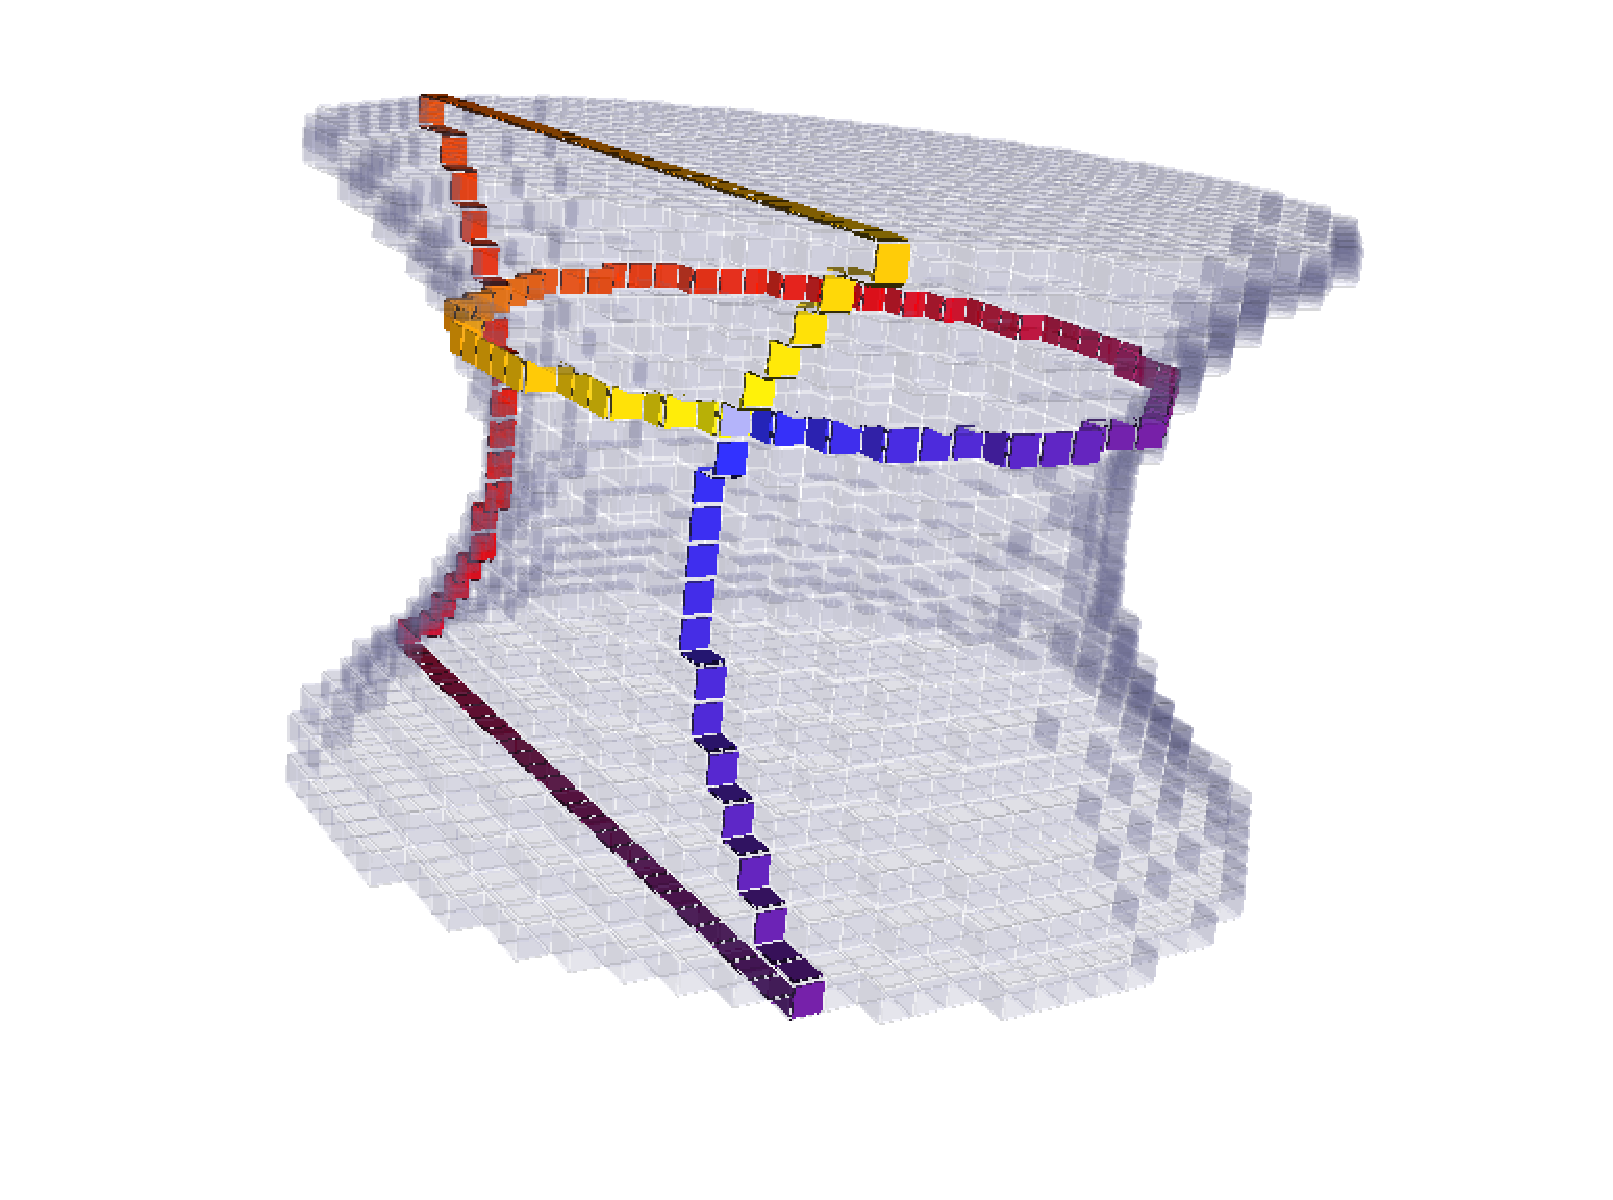
\includegraphics[width=5cm]{surfelTracking}}

    \subfigure[Normal vector computation on object
      surface]{\includegraphics[width=5.5cm]{normal}}~~ 
    \subfigure[Digital curve analysis using digital circular arc
      covering]{\includegraphics[width=7cm]{geomDCA-1024x272}}~~ 

  \subfigure[Multigrid shape definition for differential estimator
    evaluation]{\includegraphics[width=5cm]{shapes}}~~ 
    \subfigure[Volumetric Analysis with Distance
      transformation]{\includegraphics[width=4cm]{AlCaponeDistanceMap}} 
  \end{center} 
\end{figure}



 



\section*{Project Management \& Team}

\DGtal uses a github project
(\url{https://github.com/DGtal-team/DGtal})  to host the code
(using \texttt{git} as control version system) and to list open/closed
issues. The documentation is managed by \texttt{doxygen} (both user-guides and
technical documentation). 
The \DGtal project is composed of several sub-projects:
\begin{description}
  \item[{DGtal}:] the main library (classes + unit tests + example programs
    + documentation files)
\item[{DGtalTools}:] command line tools built using DGtal (multigrid shape generators,
    contour analyzers, file format converter,...)
\item[{DGtalScripts}:] scripts for developers,  class skeletons,...  
\end{description}
In order to follow and manage \DGtal developments, several
\emph{groups} have been identified. The \textbf{Editorial Board}
prepares releases, organises DGtal meetings, (\emph{David Coeurjolly,
  Jacques-Olivier Lachaud}). The \textbf{Package Managers} are
in-charge of the package design (main concepts, relationships with
other packages\ldots), and organise and check package contributions
(aka modules). Finally \textbf{Contributors} adds new features to
DGtal (classes + concept + test
      files + documentation) as a new module in a DGtal package.
\begin{center}
  \includegraphics[width=1.8cm]{liris-logo}~~~~~
  \includegraphics[width=1.8cm]{lama-logo}~~~~~
  \includegraphics[width=1.8cm]{loria-logo_new}~~~~~
  \includegraphics[width=1.8cm]{greyc-logo}~~~~~
  \includegraphics[width=1.8cm]{gipsa-logo}~~~~~
  \includegraphics[width=1.8cm]{irccyn_transparent}
\end{center}

\end{document}
